%%%%%%%%%%%%%%%%%%%%%%%%%%%%%%%%%%%%%
\chapter{Physical Layer Components}
\label{sec:physical-layer-components}
%%%%%%%%%%%%%%%%%%%%%%%%%%%%%%%%%%%%%

Now that we have a basic knowledge of the working principles behind a quantum repeater, it is time to delve a little deeper.
In this chapter, we will see how individual physical components of a quantum repeater work.





%%%%%%%%%%%%%%%%%%%%%%%%%%%%%
\section{Introduction}
\label{sec:phys_layer_intro}
%%%%%%%%%%%%%%%%%%%%%%%%%%%%%

\begin{figure}[t]
    \centering
    \includegraphics[width=0.7\textwidth]{lesson13/13-1_repeater.pdf}
    \caption[MIM link hardware.]{The MIM link. The nodes at each end are repeaters with memories, shown by the atom symbols.  The node in the middle is the Bell-state analyzer (BSA). The red circles represent photons in flight, entangled with the memories.}
    \label{fig:13-MIM-link}
\end{figure}


Fig.~\ref{fig:13-MIM-link} shows the basic MIM architecture for a quantum repeater link.
What are the individual physical components of a quantum repeater system?
We require a physical system that can be used as a suitable \textbf{\emph{quantum memory}}\index{quantum memory}, represented by the red atom symbols in the figure.
Ideally, we would like to interact with this system optically, meaning it is possible to use laser pulses to manipulate the state of the quantum memory, and make it emit photons.
The difference between classical memories and quantum memories is quite substantial.
Classical memories store 0s and 1s (classical bits), whereas quantum memories have to be able to store not only \ket{0} or \ket{1}, but also entangled state. 
This state could be a pure superposition, or it could be part of a distributed entangled state.
In fact, the latter case will be the usual scenario in our considerations.

The photons emitted from the quantum memories must be collected into an optical fiber.
We have covered optical fibers in Chapters~\ref{sec:7_waveguides}\index{optical fiber} and \ref{sec:11_long-distance} already.
Finally, we need to think how to implement the BSA in the middle.
We know what the function of a BSA is, but we have not discussed the physical components needed that can implement it.

The first half of this chapter is dedicated to Bell-state measurements.
We will discuss two different types of these measurements.
The first type is used in entanglement swapping between two quantum memories.
This Bell-state measurement is used to extend link-level entanglement to longer distances as seen in Chapter~\ref{sec:repeaters}.
The second type is photonic Bell-state measurement.
We will see that these two types of measurement have very different physical implementation, with different consequences, even though they both implement the same function.

In the latter half of this chapter, we will talk about quantum memories.
We will begin with consideration of what a good quantum memory should be like before moving to candidate systems.
We say ``candidate'' because at the moment, there is no leading physical system that is considered to be the best quantum memory. All of the existing candidate systems have their own advantages and drawbacks.


%%%%%%%%%%%%%%%%%%%%%%%%%%%%%%%%%%%%%%
\section{Bell State Measurements I}
\label{sec:bell-state-measurements-I}
%%%%%%%%%%%%%%%%%%%%%%%%%%%%%%%%%%%%%%

In this Section, we focus on the Bell state analyzer from Fig.~\ref{fig:13-MIM-link}, particularly how one can perform measurements in the Bell basis.
We have seen how to describe this measurement mathematically in Chapter~\ref{sec:4_entanglement}.
However, this tells us little about a real-world implementation.
The first step is to break down the Bell state measurement into more elementary operations in order to understand how we can implement it using a real physical system.

Let's step back a little and consider something simpler first, like measuring a single qubit in the Pauli $Z$ basis, depicted in the left panel of Fig.~\ref{fig:13-2_measurementPauli}.
The meter icon represents a measurement in the Pauli Z basis which outputs a single classical bit $c$.
The value of this classical bit can be either $+1$ or $-1$, which is normally written as $c\in\{+1,-1\}$.
For an arbitrary initial state $|\psi\rangle = \alpha |0\rangle + \beta |1\rangle$, the probability that the measurement outcome is $c=+1$ is given by $\text{Pr}(+1)=|\langle0|\psi\rangle|^2=|\alpha|^2$.
The probability that the measurement outcome is $c=-1$ is given by $\text{Pr}(-1)=|\langle1|\psi\rangle|^2=|\beta|^2$.

\begin{figure}[t]
    \centering
    \includegraphics[width=0.6\textwidth]{lesson13/13-2_measurementPauli.pdf}
    \caption[Changing the basis of measurements.]{Changing the basis of a measurement can be achieved by applying a suitable unitary to the state and then measuring in the Pauli $Z$ basis.}
    \label{fig:13-2_measurementPauli}
\end{figure}

We can also measure the qubit in the Pauli $X$ basis, as shown in the top part of the right panel in Fig.~\ref{fig:13-2_measurementPauli}.
The measurement icon includes an X to remind us that we are measuring in the Pauli $X$ basis.
The probability that we obtain $c=+1$ is $\text{Pr}(+1)=|\langle+|\psi\rangle|^2=|\alpha+\beta|^2/2$, and the probability of the outcome $c=-1$ is $\text{Pr}(-1)=|\langle-|\psi\rangle|^2=|\alpha-\beta|^2/2$.

But what if we cannot perform the Pauli $X$ measurement directly?
Sometimes, in an experiment, it is straightforward to implement a Pauli $Z$ measurement, but much less clear how to perform a measurement in a different basis.
We can still measure in the desired basis by rotating the state with an appropriate unitary and then performing a measurement in the Pauli $Z$ basis.
In the case of a Pauli $X$ measurement, the appropriate unitary is a Hadamard gate $H$, as shown in the lower part of the right panel in Fig.~\ref{fig:13-2_measurementPauli}.
The state immediately before the measurement in the Pauli $Z$ basis is
\begin{align}
    |\psi'\rangle & = H|\psi\rangle \nonumber\\
    & = \alpha |+\rangle + \beta |-\rangle \nonumber\\
    & = \frac{\alpha + \beta}{\sqrt{2}} |0\rangle + \frac{\alpha - \beta}{\sqrt{2}} |1\rangle.
\end{align}
We can immediately see that the probabilities of obtaining measurement outcomes $+1$ or $-1$ are the same as the probabilities of measuring in the Pauli $X$ basis directly.

How do we know that the unitary that is needed is the Hadamard $H$?
The trick lies in realizing that the probability of obtaining the $c=+1$ outcome via a direct Pauli $X$ measurement must be the same as first rotating the state with some unitary operation $U$ and then measuring in Pauli $Z$ basis.
Written more formally, we require that
\begin{equation}
    |\langle+|\psi\rangle|^2 = |\langle0|U^{\dagger}|\psi\rangle|^2.
    \label{eq:13-2_prob_condition}
\end{equation}
Eq.~(\ref{eq:13-2_prob_condition}) is satisfied when $\langle+|=\langle0|U^{\dagger}$, or $|+\rangle=U|0\rangle$ if you prefer to think in terms of kets rather then bras.
The same unitary $U$ must also satisfy
\begin{equation}
    |\langle-|\psi\rangle|^2 = |\langle1|U^{\dagger}|\psi\rangle|^2,
\end{equation}
that is, the probabilities of obtaining the outcome $c=-1$ via direct measurement in Pauli $X$ basis and via rotating the state before measuring in the Pauli $Z$ basis must be the same.
The unitary operation $U$ that achieves this transformation is the Hadamard $H$, as we saw in Sec.~\ref{sec:2-2_unitary_operations}.

\begin{figure}
    \centering
    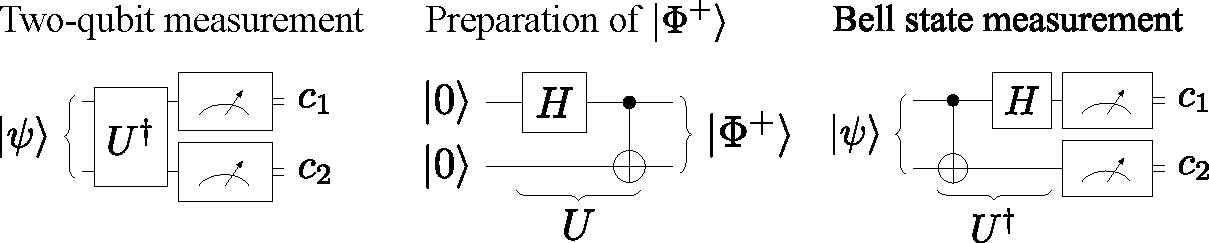
\includegraphics[width=0.9\textwidth]{lesson13/13-2_measurementBell.pdf}
    \caption[Bell state measurement via Pauli Z measurements.]{Performing the Bell state measurement can be achieved by the right unitary $U$ followed by two measurements in the Pauli $Z$ basis.}
    \label{fig:13-2_measurementBell}
\end{figure}

Transforming the measurement basis by applying a suitable unitary operation on the state does not stop with single qubits but works for multi-qubit measurements as well.
Let's turn our attention to the Bell state measurement.
What is the two-qubit unitary that we must apply such that subsequent measurements of both qubits in the Pauli $Z$ basis have the same effect as a Bell state measurement?
We can apply the same technique that we used in the case of single-qubit Pauli $X$ measurement and look for a unitary $U$ which satisfies
\begin{equation}
    |\langle\Phi^+|\psi\rangle|^2 = |\langle00|U^{\dagger}|\psi\rangle|^2,
\end{equation}
where $|\psi\rangle$ is now an arbitrary two-qubit state, as depicted in the left panel of Fig.~\ref{fig:13-2_measurementBell}.
The outcomes of the measurements on the first and second qubit are denoted by $c_1$ and $c_2$, respectively.
We see that our desired unitary $U$ must satisfy $\langle\Phi^+| = \langle00|U^{\dagger}$, which can be expressed in the ket notation by taking the adjoint of both sides,
\begin{equation}
    |\Phi^+\rangle = U |00\rangle.
\end{equation}
This means we need to find the unitary $U$ which transforms the input $|00\rangle$ into the Bell pair $|\Phi^+\rangle = (|00\rangle + |11\rangle) / \sqrt{2}$.
This unitary operation is pictured in the middle panel of Fig.~\ref{fig:13-2_measurementBell},
\begin{equation}
    U = CNOT_{12} \cdot (H \otimes I).
    \label{eq:13-2_U}
\end{equation}
Starting from the initial state where both qubits are initialized in the $|0\rangle$, we need to apply the Hadamard operation $H$ to the first qubit, followed by a controlled-NOT gate with the first qubit being the control and the second qubit the target.
All that remains to be done is to take the adjoint of Eq.~(\ref{eq:13-2_U}),
\begin{equation}
    U^{\dagger} = (H \otimes I) \cdot CNOT_{12},
\end{equation}
which swaps the order of the Hadamard and the CNOT gates.
This is the unitary operation that we need to apply to the state \ket{\psi} in order to be able to perform a Bell state measurement using measurements in the Pauli $Z$ basis, as shown in the right panel of Fig.~\ref{fig:13-2_measurementBell}.
This trick is very useful in both quantum computation and quantum communication.

This form of the Bell-state measurement is suited for quantum memories.
The three operations required are the Hadamard gate, CNOT gate, and measurement in Pauli $Z$ basis.
A candidate system for a quantum memory usable in a quantum repeater must be able to implement all three of these operations.



%%%%%%%%%%%%%%%%%%%%%%%%%%%%%%%%%%%%%%%%%
\section{Bell State Measurements II}
\label{sec:bell-state-measurements-II}
%%%%%%%%%%%%%%%%%%%%%%%%%%%%%%%%%%%%%%%%%

In this section, we will turn our attention to Bell-state measurement of photonic qubits.
We will see that even though the abstract function of the BSA is the same as entanglement swapping, the implementation differs substantially from the case of quantum memories discussed in Sec.~\ref{sec:bell-state-measurements-I}.
The implementation scheme depends on the particular encoding chosen.
We will consider the case of encoding the state of a qubit using the photon's polarization.
There are two reasons for this choice.
First, it is intuitive and simple to visualize so it makes a good pedagogical example.
Second, it is one of the most commonly used encodings in real experiments.

In this encoding, a qubit in the state \ket{0} is represented as a single photon that is polarized in the horizontal direction, which we write as \ket{H}.
The other computational basis state \ket{1} is represented as a single photon polarized in the vertical direction, and we write \ket{V}.

\begin{figure}[t]
    \centering
    \includegraphics[width=0.6\textwidth]{lesson13/13-3_PBS.pdf}
    \caption[A polarizing beam splitter (PBS).]{The action of a polarizing beam splitter (PBS).  The vertical rays represent vertically polarized light \ket{V}, while the diagonal rays represent horizontally polarized light \ket{H}.  The direction of propagation, red arrows, is normal to the \ket{H}-\ket{V} plane.}
    \label{fig:13-PBS}
\end{figure}

The first question that we should ask is, ``how do we implement a Pauli $Z$ measurement with this encoding?''
We need to distinguish horizontal and vertical polarizations.
This can be done with a piece of crystal called a \emph{\textbf{polarizing beam splitter}} (PBS)\index{polarizing beam splitter (PBS)}, as shown in Fig.~\ref{fig:13-PBS}.
A PBS transmits light of horizontal polarization only, and reflects vertically-polarized light.
An incident beam of arbitrary polarization gets split into two beams by the PBS.
The relative strength of the two beams depends on the polarization of the input light.
The PBS is not creating or changing polarization, but rather sorting the input light into the two categories.
Thinking in terms of computational states, we now have two beams, one for our \ket{0} and one for our \ket{1}.

\begin{figure}[t]
    \centering
    \includegraphics[width=0.7\textwidth]{lesson13/13-3_PBS_measure.pdf}
    \caption[A polarizing beam splitter (PBS) measuring a qubit.]{A PBS measuring an arbitrary photonic qubit in the \{$|H\rangle$, $|V\rangle$\} basis.}
    \label{fig:13-PBS-measure}
\end{figure}

Assume that we have a single photon incident onto the PBS.
We can determine which output path was taken by the photon by placing two detectors into the two possible output paths, as shown in Fig.~\ref{fig:13-PBS-measure}.
If the photon is horizontally polarized, it gets transmitted through the polarizing beam splitter.
It has no chance of being reflected and gets detected by the detector placed in the transmitted path with probability one.
This represents our measurement outcome of $+1$.
On the other hand, if the initial photon is vertically polarized, it always gets reflected and travels down into the bottom detector.
In that case, the probability of the outcome $-1$ is 1, and the probability of the outcome $+1$ is always 0.

What happens if we put in a superposition of the two linear polarizations, as in Fig.~\ref{fig:13-PBS-measure}?
Our input state is given by $\alpha\ket{H} + \beta \ket{V}$.
The photon has a chance to get transmitted, with probability given by $|\alpha|^2$, and it also has a chance to get reflected and travel down into the other detector corresponding to the measurement outcome $-1$ (bottom), with probability of $|\beta|^2$.
This shows how this arrangement implements a measurement in the Pauli $Z$ basis.

We have seen in the previous step that for a Bell-state measurement, we need two measurements in the $Z$ basis and a suitable unitary preceding the measurements.
We have just learned that $Z$ measurements can be implemented with a single PBS and two detectors.
Two $Z$ measurements will therefore require two PBS and four detectors.
The last remaining ingredient that is needed is the unitary transformation changing the basis of the measurements.
This unitary is given by a regular, non-polarizing, beam splitter as pictured in Fig.~\ref{fig:13-BSA-clicks}.

Let's investigate the behavior of the optical arrangement in Fig.~\ref{fig:13-BSA-clicks}.
Assume we have two incoming photons, one coming from the top and one coming from the left, arriving at the regular beam splitter simultaneously.
A complete analysis requires a lot more quantum optics than we have studied so far, so instead of the full derivation, here we will give the result.
Depending on which of the four detectors click, we may learn which Bell-state has been measured.
Let's see what the different patterns are.

\begin{figure}[t]
    \centering
    \includegraphics[width=0.6\textwidth]{lesson13/13-3_BSA_clicks.pdf}
    \caption[A four-detector Bell-state analyzer (BSA).]{A BSA measuring a pair of photonic qubits, one arriving at the initial beam splitter from above and one from the left.  Different click patterns on the four detectors may confirm projection of the pair into a Bell state, or be ambiguous.}
    \label{fig:13-BSA-clicks}
\end{figure}

If we get a joint detection in detectors $D_1$ and $D_4$, meaning that both detectors click, then we have implemented a successful Bell measurement, and the outcome corresponds to the projection onto the state \ket{\Psi^-}.
If we get a joint detection in $D_2$ and $D_3$, then we can also say that we have implemented a successful Bell measurement, and the result corresponds to the state \ket{\Psi^-}.
A different pattern is a joint detection at the two detectors in the lower branch of our Bell-state analyzer (both $D_1$ and $D_2$ click), from which we can conclude that we have a state \ket{\Psi^+}, corresponding to another successful Bell measurement.
Equally, if both detectors in the right branch of our Bell-state analyzer ($D_3$ and $D_4$) click, then we can also conclude that we have a Bell-state \ket{\Psi^+}.

It is also possible that both photons travel into a single detector. (Detection in any of the four detectors is equally probable.) However, because more than one Bell state can result in this happening, the answer we get is ambiguous: we cannot say that whether we have \ket{\Phi^+} or \ket{\Phi^-}.
This is a problem because we cannot fully implement a Bell-state measurement.
We cannot distinguish all four Bell states, only two of them, \ket{\Psi^+} and \ket{\Psi^-}.
Using the arrangement in Fig.~\ref{fig:13-BSA-clicks}, we can only implement a partial Bell-state measurement.

\begin{table}
    \setcellgapes{3pt}
    \renewcommand\theadfont{}
    \makegapedcells
    \centering
    \begin{tabular}{cccc}
    \hline
        \textbf{Pattern}  & \textbf{Result} & \textbf{Reason} & \textbf{Action} \\
        \hline
        $D_1$ and $D_4$ & \ket{\Psi^-} & & \textcolor{mygreen}{keep} \\
        $D_2$ and $D_3$ & \ket{\Psi^-} & & \textcolor{mygreen}{keep} \\
        $D_1$ and $D_2$ & \ket{\Psi^+} & & \textcolor{mygreen}{keep} \\
        $D_3$ and $D_4$ & \ket{\Psi^+} & & \textcolor{mygreen}{keep} \\
        single click & \ket{\Phi^\pm}  & two photons together/only one arrived & \textcolor{myred}{discard} \\
        no click & N/A & photons lost/detection failure & \textcolor{myred}{discard} \\
        other pattern & N/A & detection error & \textcolor{myred}{discard} \\
        \hline
    \end{tabular}
    \caption[Four-detector BSA click patterns.]{4-detector BSA click patterns and their meaning, based on Fig.~\ref{fig:13-BSA-clicks}.}
    \label{tab:bsa-clicks}
\end{table}

A complete, unambiguous Bell-state measurement cannot always be successfully implemented with linear optics.
In fact, even with 100\% probability of receiving both photons, the maximum probability of a successful Bell measurement is limited to only 50\% at most.
Of course, as we saw when discussing the loss of photons in fiber, the loss of one or both photons is highly probable, increasing the ambiguity of interpreting the result of one click.
These cases (along with the case where something goes wrong in the hardware) are summarized in Tab.~\ref{tab:bsa-clicks}. 
Moreover, we have to take into account that the two photons coming into our Bell-state analyzer have to be synchronized.
If they come in so close together that two detectors click \emph{almost} simultaneously, but not close enough that the photons are truly indistinguishable, we may misinterpret the result.
The Bell-state measurement has failed and we did not establish entanglement between the network nodes, but may not realize it; when we accumulate statistics about the link, this results in lowered fidelity.




%%%%%%%%%%%%%%%%%%%%%%%%%%%%%%%%%%%%%%%
\section{Stationary and flying qubits}
\label{sec:statinary-and-flying-qubits}
%%%%%%%%%%%%%%%%%%%%%%%%%%%%%%%%%%%%%%%

Let's begin by considering the basic requirements for a good quantum memory, known as \textbf{\emph{DiVincenzo criteria}}\index{DiVincenzo criteria}.
These criteria were introduced in the context of quantum computation, but they also apply in the context of quantum networking, with slightly different emphasis on which ones are important.
The extended list of these criteria, with the first five for quantum computing and the latter two for quantum communication, is as follows,
\begin{enumerate}
    \item A well-defined qubit.
    \item The qubit can be initialized.
    \item Long lifetime.
    \item Universal gate set.
    \item Efficient measurement.
    \item Convert or entangle stationary and flying qubits.
    \item Able to carry flying qubits long distances.
\end{enumerate}

If we want to build a good quantum computer, we need a \textbf{\emph{well-defined qubit}}.
Qubits do not come for free in nature.
Most naturally occurring systems have a complicated energy level structure.
In order to have a well-defined qubit, we must be able to take a system for which we can address two of those energy levels, distinguish them and control them as a pair, without slipping into the other energy levels.
(Sometimes a third level is used as a temporary state to achieve certain effects such as emitting a photon, but the computation is done by restricting actions to the two levels we want to use.)

Second, we need to be able to \textbf{\emph{initialize}} this qubit.
Initialization is important because knowing the initial state of the system is crucial for computation.
Without reliable initialization, we would always get a different answer to out problem.
(This initialization also sometimes involves the temporary use of a third state.)

Third, the qubits need to have \textbf{\emph{long lifetimes}}. This means that the state of qubit, particularly a superposition state, stays stable for a sufficiently long time such that the required operations can be applied to it.
Long lifetimes allow us to carry out longer quantum computations, which we need if we want to solve harder problems.
This criterion is especially important in quantum networking, as we will see below.

Fourth, we must be able to implement a \textbf{\emph{universal set of gates}}.
The physical system implementing a qubit dictates how we can interact with and manipulate the state of the qubit.
Typically this is done with a set of laser pulses in the case of ion qubits sitting in a magnetic trap, or with microwave pulses in the case of superconducting qubits.
If is usually difficult to implement an arbitrary operation with a single pulse.
Luckily, any complicated operation can be broken down and approximated by a series of simpler operations.
Usually, it is enough to be able to implement simple rotations of single qubits and apply entangling operations between two qubits.

Fifth, we need \textbf{\emph{efficient measurements}}.
Just carrying out transformations of the state in a quantum manner is not enough.
We must extract the information from the physical system at the end of the quantum computation.
The measurements process should be accurate with low probability of error, and should be able to be performed in a timely manner.

In the context of quantum communication, we have two more requirements to consider.
The first of these is \textbf{\emph{conversion or entanglement }}between stationary and flying qubits, which we already saw earlier in this chapter.
Stationary qubits are those qubits that are sitting in the quantum network nodes, loaded into the quantum memories. 
Flying qubits are those qubits that are used for entanglement swapping in the BSAs to create link level entanglement between between the quantum memories.
We must be able to entangle photons (the flying qubits) with the stationary qubits inside the memories, but also we must be able to use entanglement swapping to create end-to-end entanglement.

Lastly, we also must be able to \textbf{\emph{transport flying qubits}} over long distances.
The physical system used for flying qubits needs to be robust enough to survive the long journey between the network nodes.
It is for this reason that photons are a good physical system used for communication between distant nodes.

In this Section, we will look at the memory lifetime, and the two communications requirements.

We mentioned already that the ratio of gate speed to memory lifetime is important in quantum computing.
Longer memory lifetimes and shorter gate speeds let us carry out more complex calculations
In the context of quantum communications, we often store qubits for long periods of time without acting on them, as we await messages from partners in the network.
Therefore, what is more important is not the gate speed itself, but the ratio of memory lifetime to communication time, 
provided that the gate time is short compared to the \textbf{\emph{round trip time (RTT)}}\index{rount trip time (RTT)}. 

Let's consider how we establish link level entanglement using the MIM architecture.
The quantum memories emit photons entangled with their respective memory.
These photons are guided by the optical fiber to the BSA, where they get get measured in the Bell basis.
The BSA then communicates the outcome of the measurement back to the  network nodes via a classical message.
The total time needed for the emitted photon to reach the BSA and the classical message to reach the node holding the quantum memory is the round trip time~\footnote{RTT for a link can be node to BSA and back again in some contexts, or all the way memory node to memory node and back again in others. It should be clear from the context which we mean.}.
If the memory lifetime is shorter than the RTT, then we cannot reliably establish the link-level entanglement.
Even if we successfully perform the Bell-state measurements on the photon pairs at the BSA, by the time the return messages are received, our memories will have decohered and are not useful anymore.

Table~\ref{tab:rtt} shows some typical RTTs for various length of fiber.
The speed of light in a fiber is approximately $0.2$ meters per nanosecond, so if our nodes are one kilometer apart, one round trip from one node to the other and back takes 10 microseconds. For a hundred kilometers, it increases to one millisecond, and for ten thousand kilometers it goes all the way up to 100 milliseconds (0.1 seconds) per round trip time.
The values \textbf{\emph{five nanoseconds per meter one way}} and \textbf{\emph{10 microseconds per km round trip}} are easy metrics to remember.

\begin{table}
    \setcellgapes{3pt}
    \renewcommand\theadfont{}
    \makegapedcells
    \centering
    \begin{tabular}{cc}
    \hline
    \textbf{distance (km)}  & \textbf{RTT in fiber} \\
    \hline
    1     & $10\mu$sec \\
    10    & $100\mu$sec \\
    100   & $1$msec \\
    1,000 & $10$msec \\
    10,000 & $100$msec \\
    \hline
    \end{tabular}
    \caption{Round trip times in optical fiber.}
    \label{tab:rtt}
\end{table}

What processes degrade the quantum memories?
The two main processes are \textbf{\emph{energy relaxation}}\index{energy relaxation} and \textbf{\emph{dephasing}}\index{dephasing}.
They are characterized by two different time scales, referred to as the $T_1$ time\index{$T_1$ time} scale and the $T_2$ time\index{$T_2$ time} scale, respectively.

Let's consider the energy relaxation time, given by $T_1$, first.
The two states of the physical system encoding the qubit often have different energies.
All physical systems have the tendency to try and seek the lowest energy state.
So a system initialized in the excited state will not stay there indefinitely, eventually it will lose energy and transition to a state of lower energy.
Typically, the lower-energy state is chosen to encode a \ket{0}, while the higher-energy state encodes a \ket{1}.
Of course that choice is by convention, not an immutable fact of physics.
The relaxation time $T_1$ measures at what time scales the qubit relaxes and undergoes the transition $\ket{1}\rightarrow\ket{0}$.
It tells the probability that a qubit initialized in \ket{1} is still in that state after time $t$,
\begin{equation}
    \operatorname{Prob}(\ket{1})=e^{-t / T_1}.
\end{equation}
The probability that after $T_1$ seconds we still find our state in \ket{1} is given by $\frac{1}{e}$.

The dephasing time $T_2$ tells us about the time scale of a different decoherence process, namely the loss of phase coherence in the qubit.
Unlike the relaxation process, the qubit does not necessarily lose energy, but its phase between the states \ket{0} and \ket{1} becomes uncertain over time.
The $T_2$ time tells us how quickly superpositions are washed out and the qubit decoheres and loses its wonderful quantum properties.
If we start in an equal superposition of \ket{0} and \ket{1} (the \ket{+} state), the dephasing process spreads the Bloch vector corresponding to \ket{+} around the equator of the Bloch sphere.
The fully dephased state of the qubit is then an equal mixture,
\begin{equation}
    \rho = \frac{1}{2} ( \ketbra{+}{+}+\ketbra{-}{-} ) = \frac{1}{2} ( \ketbra{0}{0}+\ketbra{1}{1} ) = \frac{I}{2}.
\end{equation}

In Sec.~\ref{sec:3-3_density_matrices}, we saw the crucial difference between complete mixtures and equal superpositions. Here, if we prepare the state in the pure state, after some time $t$ we will have the mixed state,
\begin{equation}
    \rho = P |+\rangle\langle+| + (1-P)\frac{I}{2} \quad \text{, where }  P=e^{-t / T_2}.
\end{equation}
With probability $P$, the state of the qubit will still be the initial \ket{+}, and with probability $1-P$, it will have decohered into a completely mixed state.

Both of these processes, the relaxation process and the dephasing process, are \textbf{\emph{Poisson processes}}\index{Poisson process}.
It is a little bit ironic since we are talking about memories, but these processes are also called \textbf{\emph{memoryless decay processes}}\index{memoryless decay process}, meaning that their past history does not matter, only their current state.

Now that we have talked about the lifetimes of memories, why they are important, and given some characteristic time scales for long-distance communication, let's address the question of how atoms can be entangled with photons at the physical level.

\begin{figure}[t]
    \centering
    \includegraphics[width=0.7\textwidth]{lesson13/13-4_memory-first.pdf}
    \caption[First idea for memory.]{Our first idea for a memory qubit is to use two energy levels of a system, such as ground and excited states of an atom.}
    \label{fig:13-memory-first}
\end{figure}

First we should consider what states of the atom represent the qubit basis states \ket{0} and \ket{1} in the quantum memory?
Natural choice, though not the only one, for the state \ket{0} is to use the ground state of the atom, denoted by \ket{\textrm{g}}.
The other computational basis state of the qubit, \ket{1}, is then represented by one of the excited states of the atom, denoted by \ket{\textrm{e}}.
Fig.~\ref{fig:13-memory-first} shows a two-level atom where $\ket{0}\equiv\ket{\textrm{g}}$ and $\ket{1}\equiv\ket{\textrm{e}}$.

Next, what states of the photon can we use to represent the basis states of the flying qubit?
One possibility is to use the presence or absence of a photon as a qubit, giving the representation $\ket{0}\equiv\ket{\textrm{no photon}},\ket{1}\equiv\ket{\textrm{photon}}$.
We can see in the middle panel of Fig.~\ref{fig:13-memory-first} that if the atom decays from the excited state into its ground state, it emits a photon.
The total state of the quantum memory and the flying photon undergoes the following transition,
\begin{equation}
    \ket{\textrm{e}}\ket{\textrm{no photon}} \rightarrow \ket{\textrm{g}}\ket{\textrm{photon}}.
    \label{eq:memory-photon-emit}
\end{equation}
The summary of the representations for the quantum meory and the flying qubits is shown in Tab.~\ref{tab:physical_representation}.
\begin{table}
    \setcellgapes{3pt}
    \renewcommand\theadfont{}
    \makegapedcells
    \centering
    \begin{tabular}{ccc}
    \hline
    & \textbf{quantum memory} & \textbf{flying qubit} \\
    \hline
    \textbf{physical system} & two-level atoms & emitted photons \\
    \boldmath\ket{0} & \ket{\textrm{g}} & \ket{\textrm{no photon}} \\
    \boldmath\ket{1} & \ket{\textrm{e}} & \ket{\textrm{photon}}\\
    \hline
    \end{tabular}
    \caption{Physical representation for the quantum memory and the flying qubits.}
    \label{tab:physical_representation}
\end{table}

We may now ask whether the emitted photon is entangled with the memory.
We saw in Eq.~\ref{eq:memory-photon-emit} that if the atom is prepared in the excited state \ket{\textrm{e}}, the memory-photon total state is not entangled.
We may try a different approach of initializing the atom in a superposition state $(\ket{\textrm{g}}+\ket{\textrm{e}})/\sqrt{2}$.
Let's write out the total memory-photon state step-by-step,
\begin{align}
    \frac{1}{\sqrt{2}}\left( \ket{\textrm{g}}+\ket{\textrm{e}} \right) \ket{\textrm{no photon}} & = \frac{1}{\sqrt{2}} \left( \ket{\textrm{g}}\ket{\textrm{no photon}} + \ket{\textrm{e}}\ket{\textrm{no photon}} \right) \nonumber\\
    & \rightarrow \frac{1}{\sqrt{2}} \left( \ket{\textrm{g}}\ket{\textrm{no photon}} + \ket{\textrm{g}}\ket{\textrm{photon}} \right) \nonumber\\
    & = \frac{1}{\sqrt{2}} \ket{\textrm{g}} \left( \ket{\textrm{no photon}} + \ket{\textrm{photon}} \right)
    \label{eq:memory-photon-superpostion}
\end{align}
We see that the atom has a 50\% probability to be found in the ground state initially, where it cannot emit any energy.
In that case, our photonic qubit will be in the \textbf{\emph{no photon}} state.
The atom also has a 50\% probability of being in the excited state, from where it can emit a photon.
The final state of the photon is a superposition of both being and not being emitted.
The initial superposition of the atom has been transferred to the photon.
However, we can clearly see from Eq.~(\ref{eq:memory-photon-superpostion}) that the memory is entangled with the flying photon.

\begin{figure}[t]
    \centering
    \includegraphics[width=0.3\textwidth]{lesson13/13-4_memory-second.pdf}
    \caption[Our second idea for memory.]{Our second idea for a memory qubit is to use the ground-state spin of an atom. This allows us to use a polarized photon as a flying qubit robust against loss.}
    \label{fig:13-memory-second-idea}
\end{figure}

This is a naive picture that demonstrates some of the basic principles of how stationary and flying qubits interact.
However, it suffers from a few important shortcomings.
The first one being the robustness of the encoding for the quantum memory.
Using the excited state \ket{\textrm{e}} to represent one of the computational basis states makes the memory susceptible to energy relaxation, characterized by the $T_1$ time.
Depending on the rate of energy relaxation and round trip times required, the state stored in the quantum memory might decohere and become useless.
Second, our choice of encoding for the flying qubit is not suitable due to the attenuation of light in fiber. 
If we are waiting for a message at the end of the fiber and we do not receive a photon, we cannot be sure if the original message was really \ket{\textrm{no photon}} (\ket{0}), or if the initial message was \ket{\textrm{photon}} (\ket{1}) and the photon just got lost along the way.
To fix these two problems, we will now introduce a slightly more complex version of the atom for the quantum memory and a less ambiguous encoding for the flying qubit.

Figure~\ref{fig:13-memory-second-idea} shows the new atomic structure for quantum memory.
The ground state is now degenerate~\footnote{Meaning ``having the same energy''; no moral weakness implied.}, and spanned by two orthogonal states.
The two ground states are distinguished by their spin.
One is spin\index{spin} up \ket{\uparrow}, and the other is spin down \ket{\downarrow}.
Suitable encoding for the flying qubit is the linear polarization of the photon.
State \ket{0} is represented by vertical polarization \ket{V}, and \ket{1} is represented by horizontal polarization \ket{H} as we saw at the beginning of this chapter.
This new representation is summarized in Tab.~\ref{tab:physical_representation_updated}.
\begin{table}
    \setcellgapes{3pt}
    \renewcommand\theadfont{}
    \makegapedcells
    \centering
    \begin{tabular}{ccc}
    \hline
    & \textbf{quantum memory} & \textbf{flying qubit} \\
    \hline
    \textbf{physical system} & ground state spin & linear polarization \\
    \boldmath\ket{0} & \ket{\uparrow} & \ket{V} \\
    \boldmath\ket{1} & \ket{\downarrow} & \ket{H}\\
    \hline
    \end{tabular}
    \caption{New physical representation for the quantum memory and the flying qubits.}
    \label{tab:physical_representation_updated}
\end{table}

Let's see how this representation leads to an entangled memory-photon pair.
We start by preparing the atom in the excited state \ket{\textrm{e}}.
The atom has a 50-50 probability of decaying either to the spin up \ket{\uparrow} or the spin down \ket{\downarrow} ground state.
If the atom decays into the \ket{\uparrow} state, the emitted photon will be polarized in the \ket{V} state. 
If the atom decays into the spin \ket{\downarrow} state, the photon will be polarized in the \ket{H} state.
Since we do not know the polarization of the emitted photon until we measure it, the total memory-photon state is an equal superposition of the two possibilities.
We can write this transformation as
\begin{equation}
    \ket{\textrm{e}} \rightarrow \frac{1}{\sqrt{2}} \left( \ket{\uparrow}\ket{V}+\ket{\downarrow}\ket{H} \right).
\end{equation}
This is clearly an entangled state of the quantum memory and the flying qubit required by most of the link-level architectures we studied in Sec.~\ref{sec:12-2_making_link_level_rantanglement}.

\begin{figure}[t]
    \centering
    \includegraphics[width=0.7\textwidth]{lesson13/13-4_MIM_with_energy_levels.pdf}
    \caption[Physical implementation of the MIM link.]{A different view of an MIM link. On the left are the energy level diagrams for the qubits, which decay into a superposition of two states while emitting photons entangled with the memories. On the right is a large view of the Bell state analyzer with three beam splitters and four photon detectors.}
    \label{fig:13-MIM-energy}
\end{figure}

Fig.~\ref{fig:13-MIM-energy} brings this all back to a concrete representation of our Bell-state analyzer.
So far, we have discussed the BSA only abstractly but now we have a much better idea how to make it work in practice.
In the middle are the two single-mode fibers.
On the left are the two quantum memories at our two repeater nodes, separated by some distance, represented by their energy level diagrams.
Each memory is prepared initially in the excited state \ket{\textrm{e}}, which decays into one of its ground states, either spin up \ket{\uparrow} or spin down \ket{\downarrow}.
We do not know which state it decays into, leaving us with a flying photon that is entangled with its respective memory.
These flying photons travel through the single mode fibers, then hit the central beam splitter, where (if all goes well) they interfere and we perform a Bell-state measurement using the setup we discussed in Sec.~\ref{sec:bell-state-measurements-II}.
In this way, we can establish link-level entanglement between the atomic memories sitting at the ends of the link.
This concludes our discussion of the physical implementation of the MIM link architecture.
In fact out discussion applies to the MM link architecture as well, we just need to place the BSA inside one of the nodes.
Addition of a source of entangled photon pairs, such as the one we discussed in Sec~\ref{sec:4-4_spdc} would cover also the physical implementation of the MSM link architecture.






\newpage
\begin{exercises}
\exer{
\emph{Bell-state measurement revisited.}
Let's explore the quantum circuit for a Bell-state measurement in Fig.~\ref{fig:13-2_measurementBell} a bit more detail.
\subexer{
Consider the qubits to be initialized in \ket{11} state.
What are the probabilities of the four measurement outcomes?
}
\subexer{
How do the probabilities change when the input state is \ket{\Phi^+}?
}
\subexer{
What input state should be used if the desired measurement outcome is $c_1=1$ and $c_2=1$?
}
}

\exer{
\emph{Measurement in the graph-state basis.}
We have seen how to describe Bell-state measurements using the language of quantum circuits in Sec.~\ref{sec:bell-state-measurements-I}.
In this exercise, we will explore a two-qubit measurement in a different but related basis.
\subexer{
Two-qubit graph state is an entangled state that is related to the Bell states,
\begin{equation}
    \ket{G_{00}} = I \otimes H \ket{\Phi^+}.
    \label{eq:graph-state-G00}
\end{equation}
Write down the graph state \ket{G_{00}} in Dirac notation.
}
\subexer{
Just like there are four Bell states, there are four orthogonal graph states,
\begin{equation}
    \ket{G_{mn}} = Z^m \otimes Z^n \ket{G_{00}}.
\end{equation}
Write down all four of these states in Dirac notation, and verify they are orthogonal.
}
\subexer{
Draw the quantum circuit that prepares the state \ket{G_{00}}, given the input qubits are both initialized in the \ket{0} state.
}
\subexer{
Draw the quantum circuit representation for a measurement in the graph state basis.
}
}

\exer{
\emph{Round trip time and decohering memories.}
Consider the MIM link architecture with memories that are affected by depolarizing noise with $T_1=100\mu$s.
\subexer{
Assume that the state of the memory-photon immediately after the photon emission is
\begin{equation}
    \ket{\Psi}_{\textrm{mem-phot}} = \frac{1}{\sqrt{2}} \left( \ket{\uparrow}\ket{V} + \ket{\downarrow}\ket{H} \right).
\end{equation}
What is the fidelity of this state after time $t$ that the photon has spent in flight? 
}
\subexer{
Assume that the distance of the BSA to either of the memories is $d=25$ km, and that the BSA succeeds without introducing any noise.
What is the fidelity of the Bell pair shared between the quantum memories immediately after the BSA completes?
}
\subexer{
The BSA communicates the success of entanglement swapping to the nodes.
What is the fidelity of the Bell pair after the nodes receive the classical BSA message.
}
\subexer{
Consider using a better quantum memory with $T_1=10$ ms.
What is the fidelity of the memory-memory Bell pair after receiving the BSA message?
}
}



\end{exercises}

\newpage
\section*{Quiz}
  \addcontentsline{toc}{section}{Quiz}

%\section{Learning more}

\section*{Further reading chapters 11-13}
  \addcontentsline{toc}{section}{Further reading chapters 11-13}

{\bf Chapter 11}

Our discussion of mode dispersion closely followed Section 5.6 of Hecht’s textbook and we encourage you to read it for the extra details that can be found in the book.

A qualitative review of classical amplifiers (with just the right amount of technical detail) can be found here:

Emmanuel Desurvire, The Golden Age of Optical Fiber Amplifiers, \emph{Physics Today} 47, 20 (1994)~\cite{desurvire1994golden}.

Unfortunately, this article is behind a paywall so you will have to use your university’s online system to access it.

{\bf Chapter 12}

Quantum repeaters are the "bread and butter" of quantum networks. The names Wolfgang D\"ur and Hans Briegel cannot be mentioned often enough in the history of repeaters. Those interested in the paper that introduced the idea of a quantum repeater (and are not scared off by maths) might have a look here:

Hans J. Briegel, Wolfgang Dür, Juan I. Cirac, Peter Zoller, Quantum repeaters: The role of imperfect local operations in quantum communication, \emph{Physical Review Letters} 81, 5932, (1998)~\cite{briegel98:_quant_repeater}.

The paper is behind a paywall and needs to be accessed through your university’s library online services.

One place to learn more is Prof. Van Meter's previous book,\\
Rodney Van Meter, \emph{Quantum Networking}, Wiley-ISTE, 2014~\cite{van-meter14:_quantum_networking}.



{\bf Chapter 13}

A great popular article about the physical layer components of quantum networks can be found here:
Dan Hurley, The quantum internet will blow your mind. Here’s what it will look like, \emph{Discover Magazine}, 2020~\cite{hurley2020quantum}.

Another fantastic review of physical layer components can be found here:

Nicolas Sangouard, Christoph Simon, Hugues de Riedmatten, Nicolas Gisin, Quantum repeaters based on atomic ensembles and linear optics, \emph{Review of Modern Physics} 83, 33, 2011~\cite{sangouard2011quantum}.

Again, the published version is behind a paywall. Be warned though, this paper starts with an excellent introduction but the technical details ramp up quickly after that and rely on good grasp of quantum optics. So if you get lost after the introduction, don’t worry. You can come back to those parts later.
